% Options for packages loaded elsewhere
\PassOptionsToPackage{unicode}{hyperref}
\PassOptionsToPackage{hyphens}{url}
\PassOptionsToPackage{dvipsnames,svgnames,x11names}{xcolor}
%
\documentclass[
  11pt,
  ignorenonframetext,
]{beamer}
\usepackage{pgfpages}
\setbeamertemplate{caption}[numbered]
\setbeamertemplate{caption label separator}{: }
\setbeamercolor{caption name}{fg=normal text.fg}
\beamertemplatenavigationsymbolsempty
% Prevent slide breaks in the middle of a paragraph
\widowpenalties 1 10000
\raggedbottom
\setbeamertemplate{part page}{
  \centering
  \begin{beamercolorbox}[sep=16pt,center]{part title}
    \usebeamerfont{part title}\insertpart\par
  \end{beamercolorbox}
}
\setbeamertemplate{section page}{
  \centering
  \begin{beamercolorbox}[sep=12pt,center]{part title}
    \usebeamerfont{section title}\insertsection\par
  \end{beamercolorbox}
}
\setbeamertemplate{subsection page}{
  \centering
  \begin{beamercolorbox}[sep=8pt,center]{part title}
    \usebeamerfont{subsection title}\insertsubsection\par
  \end{beamercolorbox}
}
\AtBeginPart{
  \frame{\partpage}
}
\AtBeginSection{
  \ifbibliography
  \else
    \frame{\sectionpage}
  \fi
}
\AtBeginSubsection{
  \frame{\subsectionpage}
}
\usepackage{amsmath,amssymb}
\usepackage{lmodern}
\usepackage{setspace}
\usepackage{iftex}
\ifPDFTeX
  \usepackage[T1]{fontenc}
  \usepackage[utf8]{inputenc}
  \usepackage{textcomp} % provide euro and other symbols
\else % if luatex or xetex
  \usepackage{unicode-math}
  \defaultfontfeatures{Scale=MatchLowercase}
  \defaultfontfeatures[\rmfamily]{Ligatures=TeX,Scale=1}
\fi
% Use upquote if available, for straight quotes in verbatim environments
\IfFileExists{upquote.sty}{\usepackage{upquote}}{}
\IfFileExists{microtype.sty}{% use microtype if available
  \usepackage[]{microtype}
  \UseMicrotypeSet[protrusion]{basicmath} % disable protrusion for tt fonts
}{}
\makeatletter
\@ifundefined{KOMAClassName}{% if non-KOMA class
  \IfFileExists{parskip.sty}{%
    \usepackage{parskip}
  }{% else
    \setlength{\parindent}{0pt}
    \setlength{\parskip}{6pt plus 2pt minus 1pt}}
}{% if KOMA class
  \KOMAoptions{parskip=half}}
\makeatother
\usepackage{xcolor}
\geometry{left = 1cm, right = 0.5cm, top = 0.5cm, bottom = 0.5cm}
\newif\ifbibliography
\setlength{\emergencystretch}{3em} % prevent overfull lines
\providecommand{\tightlist}{%
  \setlength{\itemsep}{0pt}\setlength{\parskip}{0pt}}
\setcounter{secnumdepth}{-\maxdimen} % remove section numbering
\usepackage{tikz} % highlight
\newcommand*{\yellowemph}[1]{%
\tikz[baseline]\node[rectangle, fill=yellow, rounded corners, inner sep=0.3mm,anchor=base]{#1};%
}
\titlegraphic{
\includegraphics[scale=0.05]{pictures/GlaLogo.pdf}}
\usepackage{float}
\usepackage{booktabs}
\usepackage{array}
\usepackage{longtable}
\usepackage{makecell}
\usepackage{fontawesome}
\usepackage{mathtools}
\usepackage{bbm}
\usepackage{xcolor}
\setbeamertemplate{itemize item}{$\diamond$}
\setbeamertemplate{itemize subitem}{\scriptsize$\diamond$}
\setbeamertemplate{itemize subsubitem}{\scriptsize$\gg$}
\definecolor{blue}{RGB}{0,114,178}
\definecolor{red}{RGB}{213,94,0}
\definecolor{yellow}{RGB}{240,228,66}
\definecolor{green}{RGB}{0,158,115}
\ifLuaTeX
  \usepackage{selnolig}  % disable illegal ligatures
\fi
\IfFileExists{bookmark.sty}{\usepackage{bookmark}}{\usepackage{hyperref}}
\IfFileExists{xurl.sty}{\usepackage{xurl}}{} % add URL line breaks if available
\urlstyle{same} % disable monospaced font for URLs
\hypersetup{
  pdftitle={Introductory Statistics for Economics},
  pdfauthor={Duong Trinh},
  colorlinks=true,
  linkcolor={blue},
  filecolor={Maroon},
  citecolor={Blue},
  urlcolor={Blue},
  pdfcreator={LaTeX via pandoc}}

\title{Introductory Statistics for Economics}
\subtitle{ECON1013: TUTORIAL 4}
\author{Duong Trinh}
\date{2025}
\institute{University of Glasgow}

\begin{document}
\frame{\titlepage}

\setstretch{1.5}
\begin{frame}{Intro}
\protect\hypertarget{intro}{}
\begin{itemize}
\tightlist
\item
  Duong Trinh

  \begin{itemize}
  \tightlist
  \item
    PhD Student in Economics (Bayesian Microeconometrics)
  \item
    Email: \underline{Duong.Trinh@glasgow.ac.uk}
  \end{itemize}
\end{itemize}

\vspace{3mm}

\begin{itemize}
\tightlist
\item
  ECON1013 TU07

  \begin{itemize}
  \tightlist
  \item
    Tuesday 2-3 pm
  \item
    4 sessions (28-Jan, 11-Feb, 25-Feb, 11-March)
  \end{itemize}
\item
  ECON1013-TU08

  \begin{itemize}
  \tightlist
  \item
    Tuesday 3-4 pm
  \item
    4 sessions (28-Jan, 11-Feb, 25-Feb, 11-March)
  \end{itemize}
\end{itemize}
\end{frame}

\begin{frame}{Your Attendance \& Tutorial Feedback}
\protect\hypertarget{your-attendance-tutorial-feedback}{}
\end{frame}

\hypertarget{brief-review}{%
\section{BRIEF REVIEW}\label{brief-review}}

\begin{frame}[fragile]{Hypothesis Testing}
\protect\hypertarget{hypothesis-testing}{}
\begin{verbatim}
## Warning: package 'knitr' was built under R version 4.2.3
\end{verbatim}

\begin{center}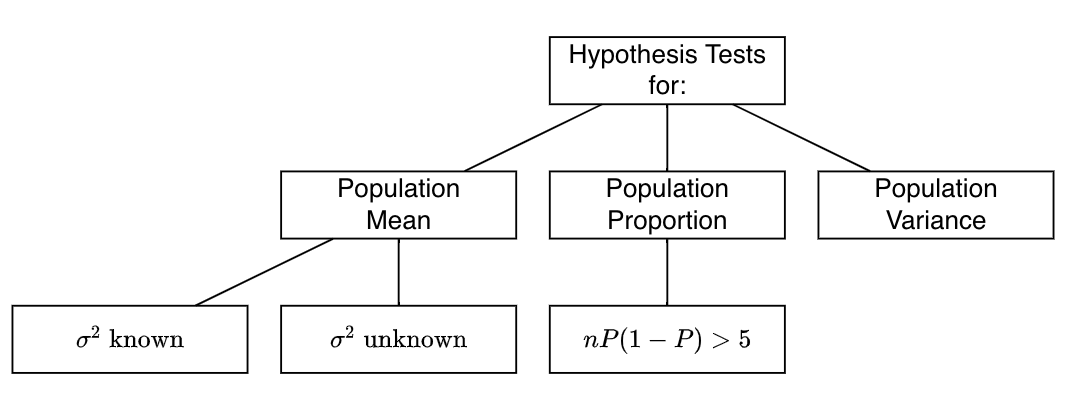
\includegraphics[width=0.9\linewidth]{../LAB3-2324/pictures/HypothesisTestObj} \end{center}
\end{frame}

\begin{frame}{Exercise 1}
\protect\hypertarget{exercise-1}{}
Using measures developed by psychologists, we have a test score
measuring a child's ability to engage in teamwork. Among childen in a
given age group, the most typical test score is 78.
\(\color{blue}{(\mu_0 = 78)}\)

This year, some children took extra sports classes in primary school. We
have data for a sample of the children who took the extra classes:

\begin{itemize}
\item
  \(\color{blue}{n=53}\)
\item
  In this sample, the average test score is \(82.3\).
  \(\color{blue}{(\bar{x} = 82.3)}\)
\end{itemize}

Suppose that the standard deviation of this population is known to be
13. \(\color{blue}{(\sigma = 13)}\)
\end{frame}

\begin{frame}{Exercise 1}
\protect\hypertarget{exercise-1-1}{}
\begin{block}{Questions}
\protect\hypertarget{questions}{}
\vspace{1mm}

\begin{enumerate}
[a)]
\tightlist
\item
  Can it be claimed at a \(1\%\) significance level that the mean test
  score among students who took extra sports differs from the typical
  value of the age group?
\end{enumerate}

\vspace{1mm}

\begin{enumerate}
[a)]
\setcounter{enumi}{1}
\tightlist
\item
  Compute the p-value associated with the observed sample mean. Explain
  how it should be interpreted.
\end{enumerate}

\vspace{1mm}

\begin{enumerate}
[a)]
\setcounter{enumi}{2}
\tightlist
\item
  Can the claim from part a) be made at the \(10\%\) significance level?
\end{enumerate}
\end{block}
\end{frame}

\begin{frame}{(1a) Can it be claimed at a \(1\%\) significance level
that the mean test score among students who took extra sports differs
from the typical value of the age group?}
\protect\hypertarget{a-can-it-be-claimed-at-a-1-significance-level-that-the-mean-test-score-among-students-who-took-extra-sports-differs-from-the-typical-value-of-the-age-group}{}
Hypothesis Testing procedure includes 5 steps:

\begin{itemize}
\tightlist
\item
  Null hypothesis \(H_0\)
\item
  Alternative hypothesis \(H_1\)
\item
  Test statistic
\item
  Decision rule
\item
  Conclusion
\end{itemize}
\end{frame}

\begin{frame}{(1a) - State Hypotheses}
\protect\hypertarget{a---state-hypotheses}{}
\begin{itemize}
    \item [$\square$] Null hypothesis $H_0$:\\
      $H_0$: The mean test score among students who took extra sports \underline{\textit{is equal to}} the typical value of the age group\\  
    \vspace{2mm}
    \item [$\square$] Alternative hypothesis $H_1$:\\
      $H_1$: The mean test score among students who took extra sports \underline{\textit{differs from}} the typical value of the age group.\\  
    \vspace{2mm}
    \item Test statistic
    \item Decision rule
    \item Conclusion
\end{itemize}
\end{frame}

\begin{frame}{(1a) - State Hypotheses}
\protect\hypertarget{a---state-hypotheses-1}{}
Denote \(\mu\) the true population mean of test score among students who
took extra sports.

\begin{itemize}
    \item [$\square$] Null hypothesis $H_0$:\\
      $H_0$: The mean test score among students who took extra sports \underline{\textit{is equal to}} the typical value of the age group.\\  
      $H_0$: $\mu = 78$
    \vspace{2mm}
    \item [$\square$] Alternative hypothesis $H_1$:\\
      $H_1$: The mean test score among students who took extra sports \underline{\textit{differs from}} the typical value of the age group.\\  
      $H_1$: $\mu \neq 78$\\
    \vspace{2mm}
    \item Test statistic
    \item Decision rule
    \item Conclusion
\end{itemize}
\end{frame}

\begin{frame}{(1a) - State Hypotheses}
\protect\hypertarget{a---state-hypotheses-2}{}
Denote \(\mu\) the true population mean of test score among students who
took extra sports.

\begin{itemize}
    \item [$\square$] Null hypothesis $H_0$: $\mu = 78$\\
    \vspace{2mm}
    \item [$\square$] Alternative hypothesis $H_1$: $\mu \neq 78$\\
      $\Rightarrow$ This is a two-tailed test.
    \vspace{2mm}
    \item Test statistic
    \item Decision rule
    \item Conclusion
\end{itemize}
\end{frame}

\begin{frame}{(1a) - Compute Test statistic}
\protect\hypertarget{a---compute-test-statistic}{}
Denote \(\mu\) the true population mean of test score among students who
took extra sports.

\begin{itemize}
    \item [$\square$] Null hypothesis $H_0$: $\mu = 78$\\
    \vspace{2mm}
    \item [$\square$] Alternative hypothesis $H_1$: $\mu \neq 78$\\
    \vspace{2mm}
    \item [$\square$] Test statistic?
    \item Decision rule
    \item Conclusion
\end{itemize}
\end{frame}

\begin{frame}{GUIDE \faMapO}
\protect\hypertarget{guide}{}
\begin{center}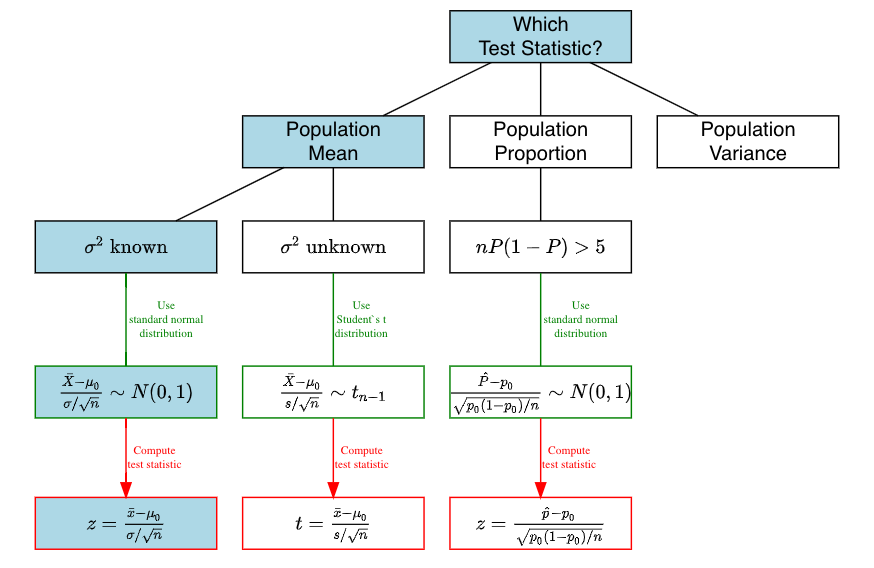
\includegraphics[width=0.9\linewidth]{../LAB3-2324/pictures/HypothesisTestsGuide-Case1} \end{center}
\end{frame}

\begin{frame}{(1a) - Compute Test statistic}
\protect\hypertarget{a---compute-test-statistic-1}{}
There is a random sample of students drawn from the population who did
extra sports, and the sample is relatively large (\(n = 53 > 25\)). This
means that the sampling distribution of the sample mean is approximately
normal. Moreover, the population standard deviation is known
(\(\sigma=13\)). Therefore, we can use a z-test. Under the null
hypothesis is true \[
Z =\frac{\bar{X}-\mu_0}{\sigma/\sqrt{n}} \sim N(0,1)
\]

We compute the realisation of the test statistic in our sample \[
z = \frac{\bar{x}-\mu_0}{\sigma/\sqrt{n}} = \frac{82.3-78}{13/\sqrt{53}} \approx 2.41
\]
\end{frame}

\begin{frame}{(1a) - Consider Decision Rule}
\protect\hypertarget{a---consider-decision-rule}{}
Denote \(\mu\) the true population mean of test score among students who
took extra sports.

\begin{itemize}
    \item [$\square$] Null hypothesis $H_0$: $\mu = 78$\\
    \vspace{2mm}
    \item [$\square$] Alternative hypothesis $H_1$: $\mu \neq 78$\\
    \vspace{2mm}
    \item [$\square$] Test statistic
$$
z = \frac{\bar{x}-\mu_0}{\sigma/\sqrt{n}} = \frac{82.3-78}{13/\sqrt{53}} \approx 2.41
$$
    \item [$\square$] Decision rule?
    \item Conclusion
\end{itemize}
\end{frame}

\begin{frame}{GUIDE \faMapO}
\protect\hypertarget{guide-1}{}
Let's answer 3 questions to find appropriate decision rule

\vspace{2mm}

\begin{enumerate}
\tightlist
\item
  Is this a two-tailed test or an one-tailed (lower-tail/upper-tail)
  test?\\
  \(\Longrightarrow\) Look again \(H_1\).
\item
  What is the \textbf{significance level} \(\alpha\)?\\
  \(\Longrightarrow\) Usually chosen to be 0.01, 0.05 or 0.10.
\item
  Is the decision rule based on
  \textcolor{green}{\textbf{critical values}} or
  \textcolor{red}{\textbf{p-value}}?\\
  \(\Longrightarrow\) Distinguish\ldots{}
\end{enumerate}
\end{frame}

\begin{frame}{(1a) - Consider Decision Rule}
\protect\hypertarget{a---consider-decision-rule-1}{}
\begin{enumerate}
\item
  We are conducting a two-tailed test (as \(H_1: \mu \neq 78\)).
\item
  The significance level \(\alpha\) = 0.01 (given in the question).
\item
  Both approaches are equivalent, we first rely on
  \textcolor{green}{\textbf{critical values}} approach.
\end{enumerate}
\end{frame}

\begin{frame}{GUIDE \faMapO}
\protect\hypertarget{guide-2}{}
\small
\begin{center}
Approach 1: \textcolor{green}{\textbf{Critical-value Test}}\\
\vspace{3mm}
\begin{tabular}{|c|c|c|}
\hline
Test & $H_1$ & Reject $H_0$ if\\
\hline
\yellowemph{Two-tailed} &  \yellowemph{$\mu \neq \mu_{0}$} & \yellowemph{$z < -z_{\frac{\alpha}{2}}$ or $ z > z_{\frac{\alpha}{2}}$}\\
\hline
Lower-tail & $\mu < \mu_{0}$ & $z < - z_{\alpha}$\\
\hline
Upper-tail & $\mu > \mu_{0}$ & $z > z_{\alpha}$\\
\hline
\end{tabular}
\end{center}

\vspace{2mm}

\begin{center}
Approach 2: \textcolor{red}{\textbf{p-value Test}}\\
\vspace{3mm}
\begin{tabular}{|c|c|c|c|}
\hline
Test & $H_1$ & p-value & Reject $H_0$ if\\
\hline
Two-tailed &  $\mu \neq \mu_{0}$ & \makecell{sum probabilities to the right \\ of $|z|$ and to the left of $-|z|$} & p-value $< \alpha$\\
    \hline
Lower-tail & $\mu < \mu_{0}$ & probability to the left of $z$ & p-value $< \alpha$\\
\hline
Upper-tail & $\mu > \mu_{0}$ & probability to the right of $z$ & p-value $< \alpha$\\
\hline
\end{tabular}

\vspace{1mm}

\footnotesize
*Note: p-value is probability of obtaining a test statistic more extreme ($\leq$ or $\geq$) than the observed sample value given $H_0$ is true.
\end{center}
\end{frame}

\begin{frame}[fragile]{(1a) - Decision Rule using Critical values
approach}
\protect\hypertarget{a---decision-rule-using-critical-values-approach}{}
For two-tailed test, reject \(H_0\) if

\[
z = \frac{\bar{x}-\mu_0}{\sigma/\sqrt{n}} < -z_{\frac{\alpha}{2}} \text{ or } z = \frac{\bar{x}-\mu_0}{\sigma/\sqrt{n}} > z_{\frac{\alpha}{2}}
\]

\vspace{2mm}

\begin{itemize}
\tightlist
\item
  Compute critical value:\\
  \(z_{\frac{\alpha}{2}} = z_{\frac{0.01}{2}} = z_{0.005} = 2.57\)\\
  (\texttt{Excel} function: \(=\text{NORM.INV}(0.995,0,1)\)).
\end{itemize}

\vspace{2mm}

\begin{itemize}
\tightlist
\item
  Compare test statistic to critical value:\\
  Notice that \(z \approx 2.41\), which is greater than \(-2.57\)
  (\(-z_{0.005}\)) and less than \(2.57\) (\(z_{0.005}\))\\
  \(\Rightarrow\) We DO NOT reject \(H_0\) at \(\alpha = 0.01\)-level.
\end{itemize}
\end{frame}

\begin{frame}{}
\protect\hypertarget{section}{}
\begin{center}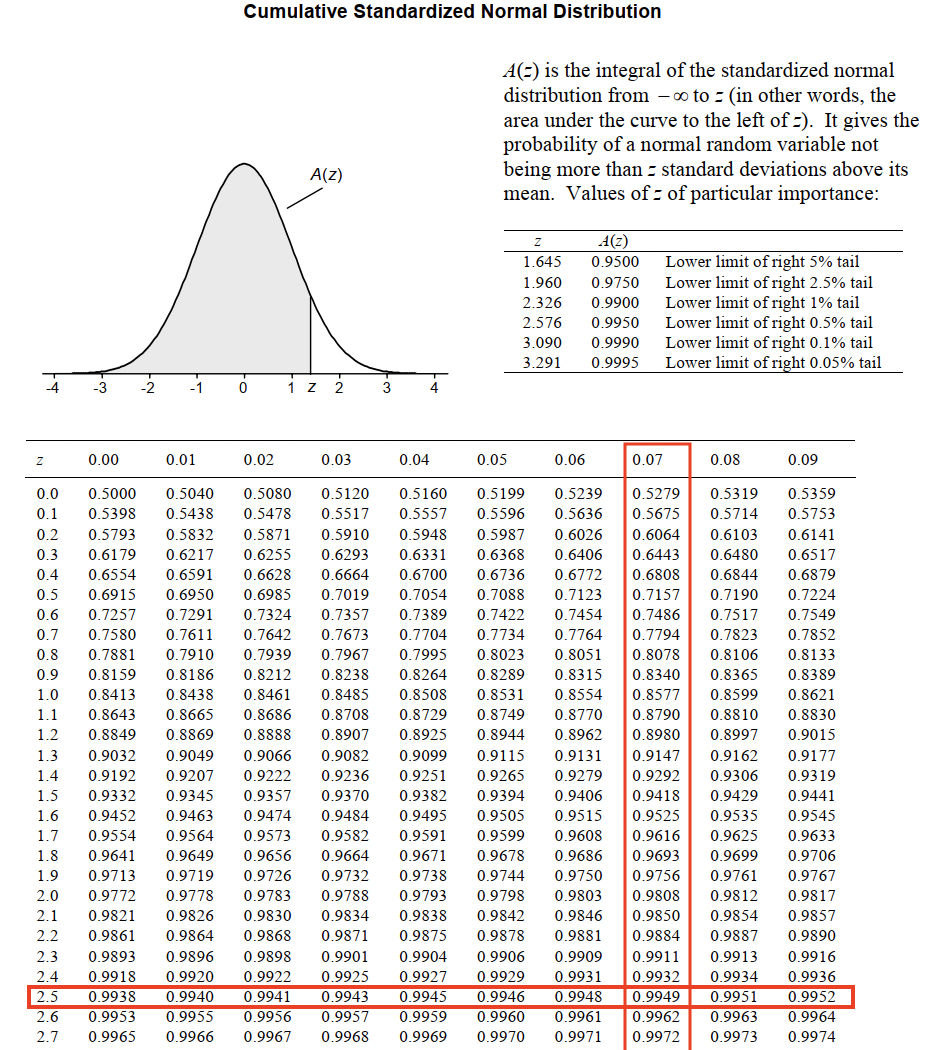
\includegraphics[width=0.7\linewidth]{pictures/Zvalue} \end{center}
\end{frame}

\begin{frame}{(1a) - Conclusion}
\protect\hypertarget{a---conclusion}{}
We DO NOT find evidence at this level suggesting that among children who
did extra sports, the mean test score would be different from the
typical test score of the age group.
\end{frame}

\begin{frame}{(1a) Hypothesis Testing}
\protect\hypertarget{a-hypothesis-testing}{}
\begin{itemize}
    \item [$\square$] \textbf{Null hypothesis} $H_0$: $\mu = 78$\\
    \vspace{2mm}
    \item [$\square$] \textbf{Alternative hypothesis} $H_1$: $\mu \neq 78$\\
    \vspace{2mm}
    \item [$\square$] \textbf{Test statistic}
\small
$$
z = \frac{\bar{x}-\mu_0}{\sigma/\sqrt{n}} = \frac{82.3-78}{13/\sqrt{53}} \approx 2.41
$$
    \normalsize
    \item [$\square$] \textbf{Decision rule} \footnotesize \textcolor{green}{*Critical values approach} \small\\
    The critical value of a two-sided z-test at the level of $\alpha=0.01$, $z_{\frac{\alpha}{2}} = z_{0.005} = 2.57$.\\
    The test statistic computed based on our sample (z=2.41) is less extreme than the critical value.\\
    $\Rightarrow$ We DO NOT reject $H_0$ at $\alpha = 0.01$.
    \normalsize
    \item [$\square$] \textbf{Conclusion}\\
    \small
    We do not find evidence at this level suggesting that among children who did extra sports, the mean test score would be different from the typical test score of the age group.
\end{itemize}
\end{frame}

\begin{frame}{(1b) Compute the p-value associated with the observed
sample mean. Explain how it should be interpreted.}
\protect\hypertarget{b-compute-the-p-value-associated-with-the-observed-sample-mean.-explain-how-it-should-be-interpreted.}{}
\small

To find the p-value associated with the observation, we are looking for
\yellowemph{the probability of observing a sample outcome as extreme or more extreme}
\yellowemph{than what we did observe, under assumption that the null hypothesis is true.}

\vspace{2mm}

This means that we are looking for the probability of finding outcomes
which are at least \(4.3\) units away from the typical value \(78\)
\((82.3-78=4.3)\). In other words, we are looking for a probability of
observing a sample average which is \emph{at least} \(82.3\) or \emph{at
most} \(73.7\).
\end{frame}

\begin{frame}{(1b) Compute the p-value associated with the observed
sample mean. Explain how it should be interpreted.}
\protect\hypertarget{b-compute-the-p-value-associated-with-the-observed-sample-mean.-explain-how-it-should-be-interpreted.-1}{}
\small

\[
\begin{aligned}
\color{red}{\mathbbm{P}}&\color{red}{(\text{Find sample outcome as extreme or more extreme than observed}\mid H_0 \text{ true})}\\
=&\underset{(1)}{\mathbbm{P}(\bar{X} \geq 82.3 \mid H_0 \text{ true})} + \underset{(2)}{\mathbbm{P}(\bar{X} \leq 73.7 \mid H_0 \text{ true})}\\
\end{aligned}
\]

\small

\[
\begin{aligned}
(1) \quad \mathbbm{P}(\bar{X} \geq 82.3 \mid H_0 \text{ true}) &= \mathbbm{P}\left(\frac{\bar{X}-\mu_0}{\sigma/\sqrt{n}} \geq \frac{82.3-\mu_0}{\sigma/\sqrt{n}} \mid H_0 \text{ true}\right)\\
&= \mathbbm{P}\left(Z \geq \frac{82.3-78}{13/\sqrt{53}}\right)\\
&= \mathbbm{P}\left(Z \geq 2.41 \right)
\end{aligned}
\] where \(Z\) follows a standard normal distribution.
\end{frame}

\begin{frame}{(1b) Compute the p-value associated with the observed
sample mean. Explain how it should be interpreted.}
\protect\hypertarget{b-compute-the-p-value-associated-with-the-observed-sample-mean.-explain-how-it-should-be-interpreted.-2}{}
\small

\[
\begin{aligned}
\color{red}{\mathbbm{P}}&\color{red}{(\text{Find sample outcome as extreme or more extreme than observed}\mid H_0 \text{ true})}\\
=&\underset{(1)}{\mathbbm{P}(\bar{X} \geq 82.3 \mid H_0 \text{ true})} + \underset{(2)}{\mathbbm{P}(\bar{X} \leq 73.7 \mid H_0 \text{ true})}\\
\end{aligned}
\] \small \[
\begin{aligned}
(2) \quad \mathbbm{P}(\bar{X} \leq 73.7 \mid H_0 \text{ true}) &= \mathbbm{P}\left(\frac{\bar{X}-\mu_0}{\sigma/\sqrt{n}} \leq \frac{73.7-\mu_0}{\sigma/\sqrt{n}} \mid H_0 \text{ true}\right)\\
&= \mathbbm{P}\left(Z \leq \frac{73.7-78}{13/\sqrt{53}} \right)\\
&= \mathbbm{P}\left(Z \leq -2.41 \right)
\end{aligned}
\] where \(Z\) follows a standard normal distribution.
\end{frame}

\begin{frame}{(1b) Compute the p-value associated with the observed
sample mean. Explain how it should be interpreted.}
\protect\hypertarget{b-compute-the-p-value-associated-with-the-observed-sample-mean.-explain-how-it-should-be-interpreted.-3}{}
\small

\[
\begin{aligned}
\color{red}{\mathbbm{P}}&\color{red}{(\text{Find sample outcome as extreme or more extreme than observed}\mid H_0 \text{ true})}\\
&=\mathbbm{P}(\bar{X} \geq 82.3 \mid H_0 \text{ true}) + \mathbbm{P}(\bar{X} \leq 73.7 \mid H_0 \text{ true})\\
&=\mathbbm{P}\left(Z \geq 2.41 \right) +\mathbbm{P}\left(Z \leq -2.41 \right)
\end{aligned}
\] where \(Z\) follows a standard normal distribution.
\end{frame}

\begin{frame}{}
\protect\hypertarget{section-1}{}
\begin{center}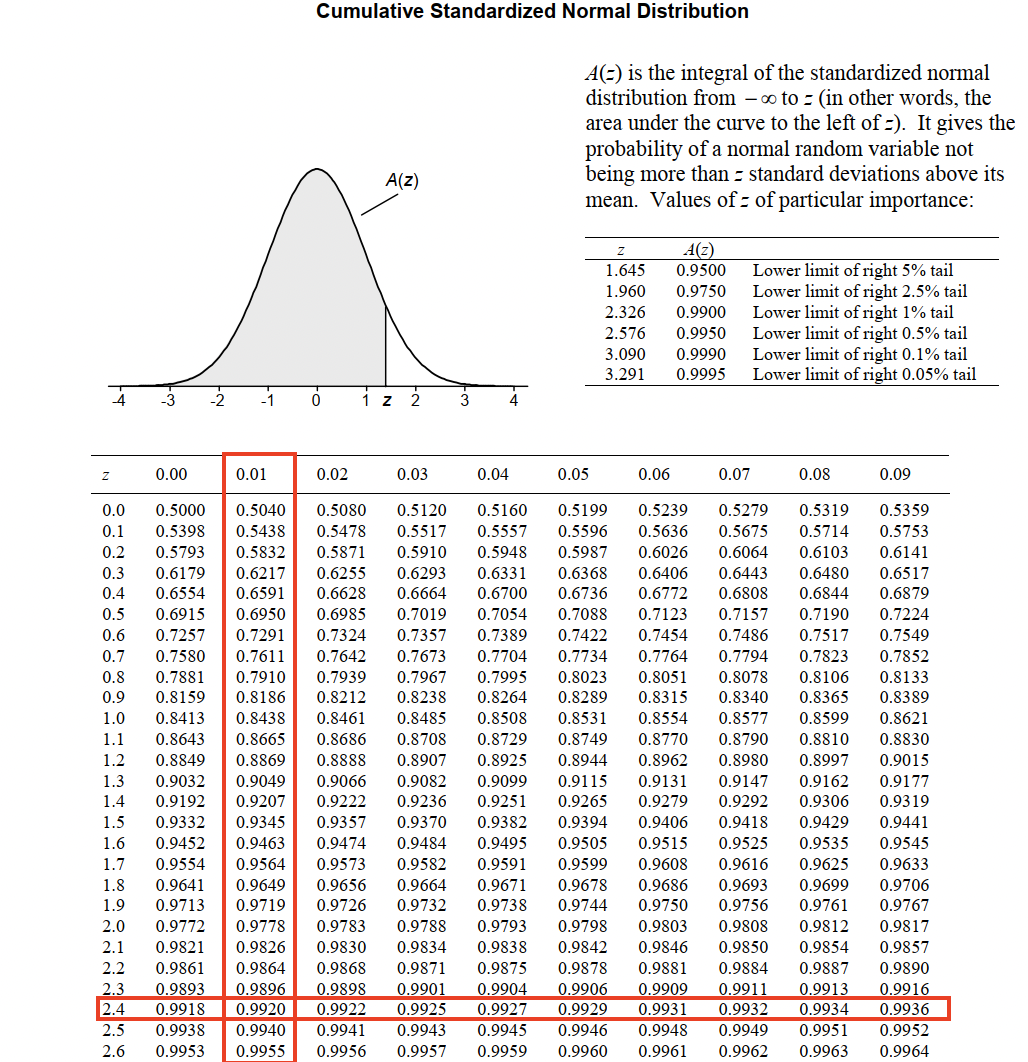
\includegraphics[width=0.8\linewidth]{pictures/Zprob} \end{center}
\end{frame}

\begin{frame}{(1b) Compute the p-value associated with the observed
sample mean. Explain how it should be interpreted.}
\protect\hypertarget{b-compute-the-p-value-associated-with-the-observed-sample-mean.-explain-how-it-should-be-interpreted.-4}{}
\small

\[
\begin{aligned}
\color{red}{\mathbbm{P}}&\color{red}{(\text{Find sample outcome as extreme or more extreme than observed}\mid H_0 \text{ true})}\\
&=\mathbbm{P}(\bar{X} \geq 82.3 \mid H_0 \text{ true}) + \mathbbm{P}(\bar{X} \leq 73.7 \mid H_0 \text{ true})\\
&= \mathbbm{P}\left(Z \geq 2.41 \right) +\mathbbm{P}\left(Z \leq -2.41 \right)\\
&= \mathbbm{P}\left(Z \geq 2.41 \right) \times 2\\
&= (1-0.992) \times 2 \\
&= 0.008 \times 2 = 0.016
\end{aligned}
\] Thus, \textcolor{red}{\textbf{p-value}} \(= 0.016\).
\end{frame}

\begin{frame}{(1b) Interpretation}
\protect\hypertarget{b-interpretation}{}
The p-value is the probability of obtaining a value of the test
statistic \textit{as extreme as or more extreme} than the actual value
obtained when the null hypothesis is true.

\yellowemph{Thus, the p-value is the \textit{smallest} significance level at which}
\yellowemph{a null hypothesis can be \textit{rejected}, given the observed sample statistic.}

A p-value larger than the significant level \(\alpha\) should be
interpreted as evidence against the rejection of the null hypothesis.
\end{frame}

\begin{frame}{}
\protect\hypertarget{section-2}{}
\begin{flushleft}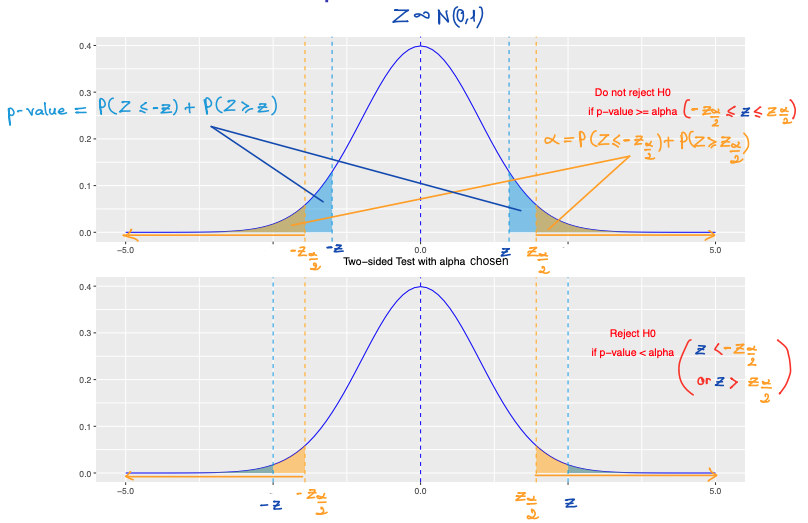
\includegraphics[width=1\linewidth]{pictures/Two-tailedTestRule} \end{flushleft}
\end{frame}

\begin{frame}{Revisit Hypothesis Testing in (1a)}
\protect\hypertarget{revisit-hypothesis-testing-in-1a}{}
\begin{itemize}
    \item [$\square$] \textbf{Null hypothesis} $H_0$: $\mu = 78$\\
    \vspace{2mm}
    \item [$\square$] \textbf{Alternative hypothesis} $H_1$: $\mu \neq 78$\\
    \vspace{2mm}
    \item [$\square$] \textbf{Test statistic}
\small
$$
z = \frac{\bar{x}-\mu_0}{\sigma/\sqrt{n}} = \frac{82.3-78}{13/\sqrt{53}} \approx 2.41
$$
    \normalsize
    \item [$\square$] \textbf{Decision rule} \footnotesize \textcolor{red}{*P-value approach} \small\\
    The p-value associated with the test statistic computed based on our sample (z=2.41) is $\mathbbm{P}\left(Z \geq 2.41 \right) +\mathbbm{P}\left(Z \leq -2.41 \right)$ = 0.016, which is larger than $\alpha = 0.01$.\\
    $\Rightarrow$ We DO NOT reject $H_0$ at $\alpha = 0.01$ (the same as Critical values approach).
    \normalsize
    \item [$\square$] \textbf{Conclusion}\\
    \small
    We do not find evidence at this level suggesting that among children who did extra sports, the mean test score would be different from the typical test score of the age group.
\end{itemize}
\end{frame}

\begin{frame}{(1c) Can the claim from (1a) be made at the \(10\%\)
significance level?}
\protect\hypertarget{c-can-the-claim-from-1a-be-made-at-the-10-significance-level}{}
\pause

Comparing the p-value \(0.016\) to \(\alpha=0.1\), we see that p-value
\(< \alpha\) (since \(0.016 < 0.1\)). We can reject the null hypothesis
at the \(10\%\) significance level.
\end{frame}

\begin{frame}{Exercise 2}
\protect\hypertarget{exercise-2}{}
\begin{itemize}
\item
  It is claimed that the average number of pieces of litter found on a
  100-meter interval on UK beaches is more than \(300\).
  \(\color{blue}{(\mu_0=300})\)
\item
  The number of items found on a 100-meter interval is known to have a
  standard deviation of \(144\). \(\color{blue}{(\sigma=144})\)
\item
  In total, data was collected from \(81\) randomly selected beaches, on
  a 100-meter interval on each beach. \(\color{blue}{(n=81})\)
\item
  We adopt the following test:

  \begin{itemize}
  \tightlist
  \item
    \(H_0\): The mean number of pieces of litter on a 100-meter interval
    on a UK beach is at least \(300\).
  \item
    \(H_1\): The mean number of pieces of litter on a 100-meter interval
    on a UK beach is less than \(300\).
  \item
    Decision rule: ``The null hypothesis will not be rejected if the
    sample mean is \(276\) items or more, and will be rejected
    otherwise.''
  \end{itemize}
\end{itemize}
\end{frame}

\begin{frame}{Exercise 2}
\protect\hypertarget{exercise-2-1}{}
\begin{block}{Questions}
\protect\hypertarget{questions-1}{}
\vspace{1mm}

\begin{enumerate}
[a)]
\tightlist
\item
  What is the level of significance \(\alpha\) (probability of a type I
  error) of this test?
\item
  Suppose that the true population mean is actually \(\mu^* = 290\).\\
  What is the probability of a type-II error (\(\beta\)) of this test in
  this case?\\
  Bonus: Try part b) with different sample sizes.
\end{enumerate}
\end{block}
\end{frame}

\begin{frame}{(2a) What is the level of significance \(\alpha\)
\qquad \qquad \qquad \qquad (probability of a type I error) of this
test?}
\protect\hypertarget{a-what-is-the-level-of-significance-alpha-probability-of-a-type-i-error-of-this-test}{}
\begin{itemize}
    \item [$\square$] \textbf{Null hypothesis} $H_0$: $\mu \geq 300$\\
    \vspace{2mm}
    \item [$\square$] \textbf{Alternative hypothesis} $H_1$: $\mu < 300$\\
    \vspace{2mm}
    \item [$\square$] \textbf{Test statistic}
\small
$$
z = \frac{\bar{x}-\mu_0}{\sigma/\sqrt{n}} = \frac{\bar{x}-300}{144/\sqrt{81}}
$$
    \normalsize
    \item [$\square$] \textbf{Decision rule}\\ \small
    This is a \textit{lower-tail} test, we reject $H_0$ if $z < - z_\alpha$. Here, the critical value $-z_\alpha$ satisfies $\mathbbm{P}(Z<-z_\alpha) = \alpha$ where $Z$ follows a standard normal distribution.\\
    $\Rightarrow$ We reject $H_0$ if:
    $$
    \frac{\bar{x}-300}{144/\sqrt{81}} < - z_\alpha \Leftrightarrow \bar{x}< - z_\alpha\cdot 144/\sqrt{81} + 300 \quad (3)
    $$
\end{itemize}
\end{frame}

\begin{frame}{GUIDE \faMapO}
\protect\hypertarget{guide-3}{}
\small
\begin{center}
Approach 1: \textcolor{green}{\textbf{Critical-value Test}}\\
\vspace{3mm}
\begin{tabular}{|c|c|c|}
\hline
Test & $H_1$ & Reject $H_0$ if\\
\hline
Two-tailed &  $\mu \neq \mu_{0}$ & $z < -z_{\frac{\alpha}{2}}$ or $ z > z_{\frac{\alpha}{2}}$\\
\hline
\yellowemph{Lower-tail} & \yellowemph{$\mu < \mu_{0}$} & \yellowemph{$z < - z_{\alpha}$}\\
\hline
Upper-tail & $\mu > \mu_{0}$ & $z > z_{\alpha}$\\
\hline
\end{tabular}
\end{center}

\vspace{2mm}

\begin{center}
Approach 2: \textcolor{red}{\textbf{p-value Test}}\\
\vspace{3mm}
\begin{tabular}{|c|c|c|c|}
\hline
Test & $H_1$ & p-value & Reject $H_0$ if\\
\hline
Two-tailed &  $\mu \neq \mu_{0}$ & \makecell{sum probabilities to the right \\ of $|z|$ and to the left of $-|z|$} & p-value $< \alpha$\\
    \hline
Lower-tail & $\mu < \mu_{0}$ & probability to the left of $z$ & p-value $< \alpha$\\
\hline
Upper-tail & $\mu > \mu_{0}$ & probability to the right of $z$ & p-value $< \alpha$\\
\hline
\end{tabular}

\vspace{1mm}

\footnotesize
*Note: p-value is probability of obtaining a test statistic more extreme ($\leq$ or $\geq$) than the observed sample value given $H_0$ is true.
\end{center}
\end{frame}

\begin{frame}[fragile]{(2a) What is the level of significance \(\alpha\)
\qquad \qquad \qquad \qquad (probability of a type I error) of this
test?}
\protect\hypertarget{a-what-is-the-level-of-significance-alpha-probability-of-a-type-i-error-of-this-test-1}{}
\begin{itemize}
\tightlist
\item
  On the other hand, the decision rule tells us that \(H_0\) is rejected
  if \(\bar{x} < 276\). Therefore, the righ-hand side quantity in
  \((3)\) has to be equal to \(276\). That means
\end{itemize}

\[
\begin{aligned}
- z_\alpha\cdot 144/\sqrt{81} + 300 &= 276\\
z_\alpha &= \frac{300-276}{144/\sqrt{81}}\\
&= 1.5
\end{aligned}
\]

\begin{itemize}
\tightlist
\item
  Thus, we are looking for \(\alpha\) such that the critical value of a
  upper-tail z-test is \(1.5\). Based on statistical table/Excel
  function \texttt{NORMSDIST()}, we will obtain
  \(\alpha = 1 - 0.9332 = 0.0668\).
\end{itemize}
\end{frame}

\begin{frame}{(2b) Suppose \(\mu^* = 290\). \hspace{9cm} What is the
probability of a type-II error (\(\beta\)) of this test?}
\protect\hypertarget{b-suppose-mu-290.-what-is-the-probability-of-a-type-ii-error-beta-of-this-test}{}
\begin{itemize}
\item
  \(\beta\) gives the probability of a type-II error, meaning the
  probability of ``maintaining a null hypothesis which is false''.
\item
  Note that if \(\mu = 290\), then the null hypothesis is false! In this
  case we would like to reject the null hypothesis.
\item
  We are thus looking for \[
  \beta = \mathbbm{P}(\text{maintain } H_0 \mid \mu = 290)
  \]
\end{itemize}
\end{frame}

\begin{frame}{(2b) Suppose \(\mu^* = 290\). \hspace{9cm} What is the
probability of a type-II error (\(\beta\)) of this test?}
\protect\hypertarget{b-suppose-mu-290.-what-is-the-probability-of-a-type-ii-error-beta-of-this-test-1}{}
\begin{itemize}
\tightlist
\item
  Using the given decision rule, \[
  \begin{aligned}
  \mathbbm{P}(\text{maintain } H_0 \mid \mu = 290) &= \mathbbm{P}(\bar{X} > 276\mid \mu = 290)\\
  &= \mathbbm{P}(\frac{\bar{X}-290}{144/\sqrt{81}} > \frac{276-290}{144/\sqrt{81}}\mid \mu = 290)\\
  &= \mathbbm{P}(Z> -0.875)\\
  &= 1 - \mathbbm{P}(Z< -0.875)\\
  &\approx 0.809
  \end{aligned}
  \]
\item
  In other words, if the true population mean would have been \(290\),
  then based on our hypothesis test we would be falsely maintaining the
  \(H_0\) more than \(80\%\) of the time.
\end{itemize}
\end{frame}

\begin{frame}{(2b) Suppose \(\mu^* = 290\). \hspace{9cm} What is the
probability of a type-II error (\(\beta\)) of this test?}
\protect\hypertarget{b-suppose-mu-290.-what-is-the-probability-of-a-type-ii-error-beta-of-this-test-2}{}
\textbf{Remark}: \(1-\beta\) is called the \textbf{power} of a test. The
power of the test depends on the true value of the population parameter.
The power of this test, if \(\mu = 290\), is around \(19\%\), which is
quite low. The power of this test increases if \(n\) grows.
\end{frame}

\end{document}
